%% Creator: Inkscape inkscape 0.91, www.inkscape.org
%% PDF/EPS/PS + LaTeX output extension by Johan Engelen, 2010
%% Accompanies image file 'GDBcommunicate.eps' (pdf, eps, ps)
%%
%% To include the image in your LaTeX document, write
%%   \input{<filename>.pdf_tex}
%%  instead of
%%   \includegraphics{<filename>.pdf}
%% To scale the image, write
%%   \def\svgwidth{<desired width>}
%%   \input{<filename>.pdf_tex}
%%  instead of
%%   \includegraphics[width=<desired width>]{<filename>.pdf}
%%
%% Images with a different path to the parent latex file can
%% be accessed with the `import' package (which may need to be
%% installed) using
%%   \usepackage{import}
%% in the preamble, and then including the image with
%%   \import{<path to file>}{<filename>.pdf_tex}
%% Alternatively, one can specify
%%   \graphicspath{{<path to file>/}}
%% 
%% For more information, please see info/svg-inkscape on CTAN:
%%   http://tug.ctan.org/tex-archive/info/svg-inkscape
%%
\begingroup%
  \makeatletter%
  \providecommand\color[2][]{%
    \errmessage{(Inkscape) Color is used for the text in Inkscape, but the package 'color.sty' is not loaded}%
    \renewcommand\color[2][]{}%
  }%
  \providecommand\transparent[1]{%
    \errmessage{(Inkscape) Transparency is used (non-zero) for the text in Inkscape, but the package 'transparent.sty' is not loaded}%
    \renewcommand\transparent[1]{}%
  }%
  \providecommand\rotatebox[2]{#2}%
  \ifx\svgwidth\undefined%
    \setlength{\unitlength}{504.52587891bp}%
    \ifx\svgscale\undefined%
      \relax%
    \else%
      \setlength{\unitlength}{\unitlength * \real{\svgscale}}%
    \fi%
  \else%
    \setlength{\unitlength}{\svgwidth}%
  \fi%
  \global\let\svgwidth\undefined%
  \global\let\svgscale\undefined%
  \makeatother%
  \begin{picture}(1,1.45089792)%
    \put(0,0){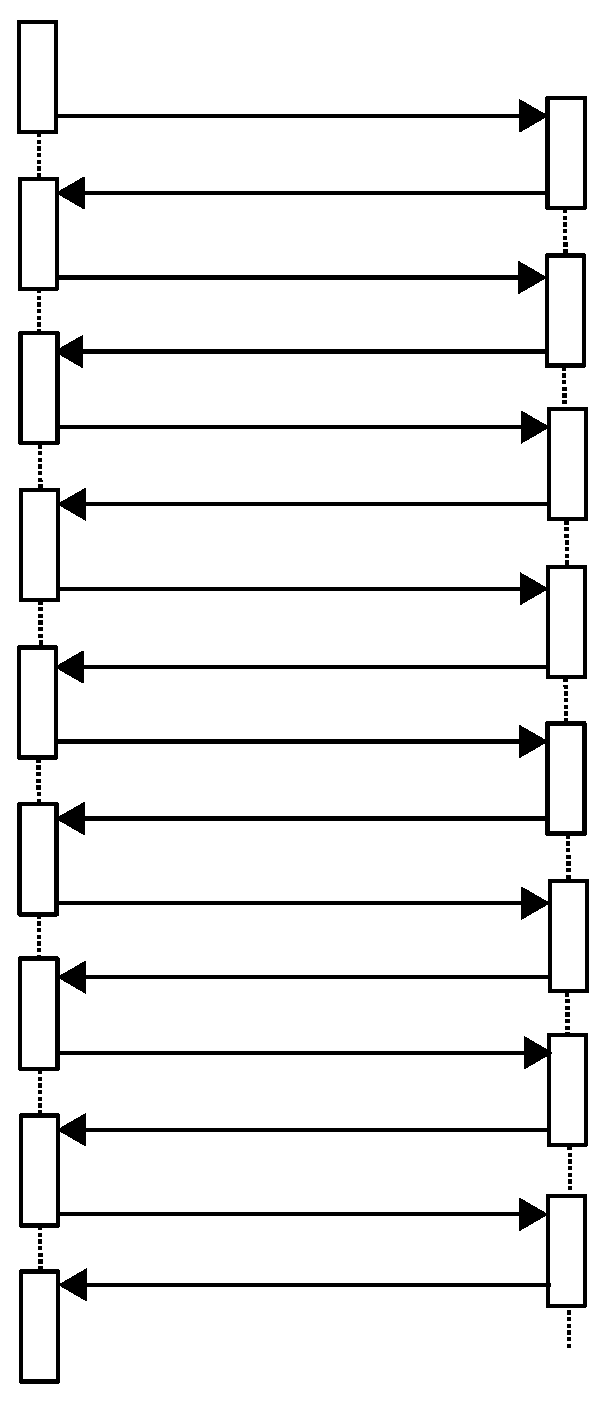
\includegraphics[width=\unitlength]{Figs/GDBcommunicate/GDBcommunicate.eps}}%
    \put(0.28895632,2.1048653){\color[rgb]{0,0,0}\makebox(0,0)[lb]{\smash{\texttt{PacketSize=120}}}}%
    \put(0.33416095,2.2398951){\color[rgb]{0,0,0}\makebox(0,0)[lb]{\smash{\texttt{qSupported}}}}%
    \put(0.44578957,1.82285535){\color[rgb]{0,0,0}\makebox(0,0)[lb]{\smash{\texttt{S05}}}}%
    \put(0.47102728,1.94651821){\color[rgb]{0,0,0}\makebox(0,0)[lb]{\smash{\texttt{?}}}}%
    \put(0.45367609,1.55762472){\color[rgb]{0,0,0}\makebox(0,0)[lb]{\smash{\texttt{OK}}}}%
    \put(0.43428917,1.69038153){\color[rgb]{0,0,0}\makebox(0,0)[lb]{\smash{\texttt{Hc-1}}}}%
    \put(0.38770689,1.27878604){\color[rgb]{0,0,0}\makebox(0,0)[lb]{\smash{\texttt{(empty)}}}}%
    \put(0.45367609,1.42154284){\color[rgb]{0,0,0}\makebox(0,0)[lb]{\smash{\texttt{qC}}}}%
    \put(0.1331809,1.004965885){\color[rgb]{0,0,0}\makebox(0,0)[lb]{\smash{\texttt{Text=0;Data=0;Bss=0;}}}}%
    \put(0.35368931,1.14128308){\color[rgb]{0,0,0}\makebox(0,0)[lb]{\smash{\texttt{qOffsets}}}}%
    \put(0.4637042,0.72651625){\color[rgb]{0,0,0}\makebox(0,0)[lb]{\smash{\texttt{OK}}}}%
    \put(0.4399683,0.87131178){\color[rgb]{0,0,0}\makebox(0,0)[lb]{\smash{\texttt{Hg-1}}}}%
    \put(0.236208,0.46355087){\color[rgb]{0,0,0}\makebox(0,0)[lb]{\smash{\texttt{000....10080000}}}}%
    \put(0.4789333,0.60834639){\color[rgb]{0,0,0}\makebox(0,0)[lb]{\smash{\texttt{g}}}}%
    \put(0.4637042,0.19357956){\color[rgb]{0,0,0}\makebox(0,0)[lb]{\smash{\texttt{OK}}}}%
    \put(0.3827329,0.3220325){\color[rgb]{0,0,0}\makebox(0,0)[lb]{\smash{\texttt{qSymbol::}}}}%
    \put(-0.15856151,2.4455925){\color[rgb]{0,0,0}\makebox(0,0)[lb]{\smash{GDB (RSP client)}}}%
    \put(0.69825017,2.4455925){\color[rgb]{0,0,0}\makebox(0,0)[lb]{\smash{\shortstack[lb]{Software server\\bridge (RSP server)}}}}%
    \put(1.167885,2.12260293){\color[rgb]{0,0,0}\makebox(0,0)[lb]{\smash{Report the supported packet  size }}}%
    \put(1.167885,1.84327822){\color[rgb]{0,0,0}\makebox(0,0)[lb]{\smash{Report the reason for target's last halt}}}%
    \put(1.167885,1.580192){\color[rgb]{0,0,0}\makebox(0,0)[lb]{\smash{Apply future operations on all threads}}}%
    \put(1.167885,1.3103437){\color[rgb]{0,0,0}\makebox(0,0)[lb]{\smash{Current thread is -1}}}%
    \put(1.167885,1.0347028){\color[rgb]{0,0,0}\makebox(0,0)[lb]{\smash{Report data offsets in the code}}}%
    \put(1.167885,0.771667){\color[rgb]{0,0,0}\makebox(0,0)[lb]{\smash{Apply future actions on all threads}}}%
    \put(1.167885,0.494383){\color[rgb]{0,0,0}\makebox(0,0)[lb]{\smash{Report all register contents}}}%
    \put(1.167885,0.203358327){\color[rgb]{0,0,0}\makebox(0,0)[lb]{\smash{Offer to provide symbol values}}}%
  \end{picture}%
\endgroup%
